% Created:  Fri 01 Aug 2014 02:02 PM
% @author Josh Wainwright
% filename: analysis.tex

\section{Cluster Analysis}
\label{sec:cluster_analysis}

Once the data has been processed and a number of clusters have been identified,
the clusters are displayed on screen in an image to allow the user to verify
them and perform further analysis. However, since the data that was used to
find the clusters is still held in memory at this point, it is useful to take
advantage of this and perform some immediate analysis and provide some
statistics regarding the clusters that were found.

There are two ways of conceptually viewing the clusters which will lead to
slightly different results when analysing them.

\begin{itemize}

	\item The first is to consider the boundary of the nodes of the quadtree
		that were considered to be part of a cluster to be the boundary of the
		cluster. This will mean that the actual cluster is likely to be
		slightly larger than the actual data points that it is comprised of,
		but is computationally simple to achieve, so fast, and can take into
		account any holes in the cluster (see below).

	\item The second way is to, once the cluster has been located, discard the
		information about the nodes themselves, and simply use them to select
		the appropriate points. This results in a set of points that are all
		considered to be spatially grouped into the same cluster. From this
		set, calculations can be performed on the real data. This method is
		guaranteed to provide information that more closely represents the
		original data, though is more computationally intensive.

\end{itemize}

\subsection{Quadtree Node Analysis}
\label{sub:quadtree_node_analysis}

Here, the nodes of the quadtree that were considered part of the cluster are
considered, rather than the points that they contain.

\subsubsection{Cluster Area}
\label{ssub:cluster_area_node}

To calculate the area of the clusters, each node in each cluster is examined.
Since the size of the node must be known, it is calculated from the quadtree
code for that node. The formula is shown in Equation~\ref{eq:node-area},
\begin{align}
	a &= \frac{1}{4^{d}} \\
	a_i &= 4^{-l_i/2}, \label{eq:node-area}
\end{align}
where $a_i$ is the area of the node $i$, $d$ is the depth in the quadtree and
$l_i$ is the length of the quadtree code of that node. For every node in the
cluster, where there are $n$ nodes, this value is summed to give the total
cluster area, $A$:
\begin{align}
	A &= \sum_{i=0}^{n} a_i.
\end{align}

\subsubsection{Cluster Perimeter}
\label{ssub:cluster_perimeter_node}

Similarly to the cluster area, the perimeter is given as a fractional value of
the length of one side of the whole image, as calculated for each node from the
quadtree code, as shown in Equation~\ref{eq:node-perimeter},
\begin{align}
	p &= \frac{1}{2^{d}} \\
	p_i &= 2^{-l_i/2}, \label{eq:node-perimeter}
\end{align}
where the symbols have the same meaning as above.

However, this simply gives the length of one side of the node for any node. In
order to calculate the perimeter of the cluster, it is not enough to simply
sum these values, as for the cluster area, since not all nodes contribute to
the perimeter. Instead, for each node, it must be decided whether it
contributes to the perimeter and how much (0, 1, 2, 3 or 4 sides), and then
increase the total perimeter by this many times the length of one side. The
total perimeter, $P$, then is given by Equation~\ref{eq:total-perimeter},
\begin{align}
	P &= \sum_{i=0}^{n} s * p_i, \label{eq:total-perimeter}
\end{align}
where $s \in \{0..4\}$. This is demonstrated in
Figure~\ref{fig:perimeter-edges} where the perimeter is simple to calculate in
case (a) as the nodes are all the same, but the size of each node must be taken
into account in case (b).

\begin{figure}[tbhp]
	\centering
	\begin{subfigure}[c]{3.5cm}
		\includegraphics[width=\textwidth]{perimeter-edges-grid.pdf}
		\caption{}\label{fig:perimeter-edges-grid.pdf}
	\end{subfigure}%
	\quad
	\begin{subfigure}[c]{3.5cm}
		\includegraphics[width=\textwidth]{perimeter-edges-quadtree.pdf}
		\caption{}\label{fig:perimeter-edges-quadtree.pdf}
	\end{subfigure}

	\caption[Perimeter size from node edge size.]{When calculating the
		perimeter of a cluster using the nodes that contribute, the size of
		each node must be taken into account. In
		case~\subref{fig:perimeter-edges-grid.pdf}, the process is simple since
		all nodes are the same size and a fractional value of 3.5 is
		calculated. For case~\subref{fig:perimeter-edges-quadtree.pdf}, the
		steps are 25 lengths of size $\rfrac{1}{8}$ and 6 lengths of size
		$\rfrac{1}{16}$ which gives the same result,
		3.5.}\label{fig:perimeter-edges}

\end{figure}

Within the cluster, \emph{holes} occur where a node is, or number of nodes are,
surrounded on all sides by the same cluster. An example can be seen in
Figure~\ref{fig:roundness}. Unfortunately, these are included in the
calculation of the perimeter and so, where holes exist in a cluster, the actual
perimeter is slightly smaller than that calculated.

\subsubsection{Cluster Roundness}
\label{ssub:Cluster_Roundness}

A potentially useful measure of a cluster is its \emph{roundness}. This
describes the extent to which the area and perimeter of the cluster resemble a
circle. The available values of roundness are from 0, meaning a perfect line
with no area but finite perimeter, to 1, being a perfect circle. The equation
to determine roundness, Equation~\ref{eq:roundness}, is defined such that it is
a unit-less ratio of area and perimeter, such that a circle has roundness 1.
The derivation of Equation~\ref{eq:roundness} is found in
Appendix~\ref{app:roundness_derivation}.

\begin{align}
	R &= \sqrt{\frac{4\pi A}{p^2}} \label{eq:roundness}
\end{align}

The clusters that are found for data sets \texttt{palm-1.txt} and
\texttt{palm-2.txt} are shown in Figure~\ref{fig:roundness}. The roundness
values for the clusters for these data are very different,
Figure~\ref{fig:roundness-long.png} has an average $R=0.350$ whereas
Figure~\ref{fig:roundness-round.png} has an average $R=0.446$.

\begin{figure}[tbhp]
	\centering
	\begin{subfigure}[b]{4.2cm}
		\fbox{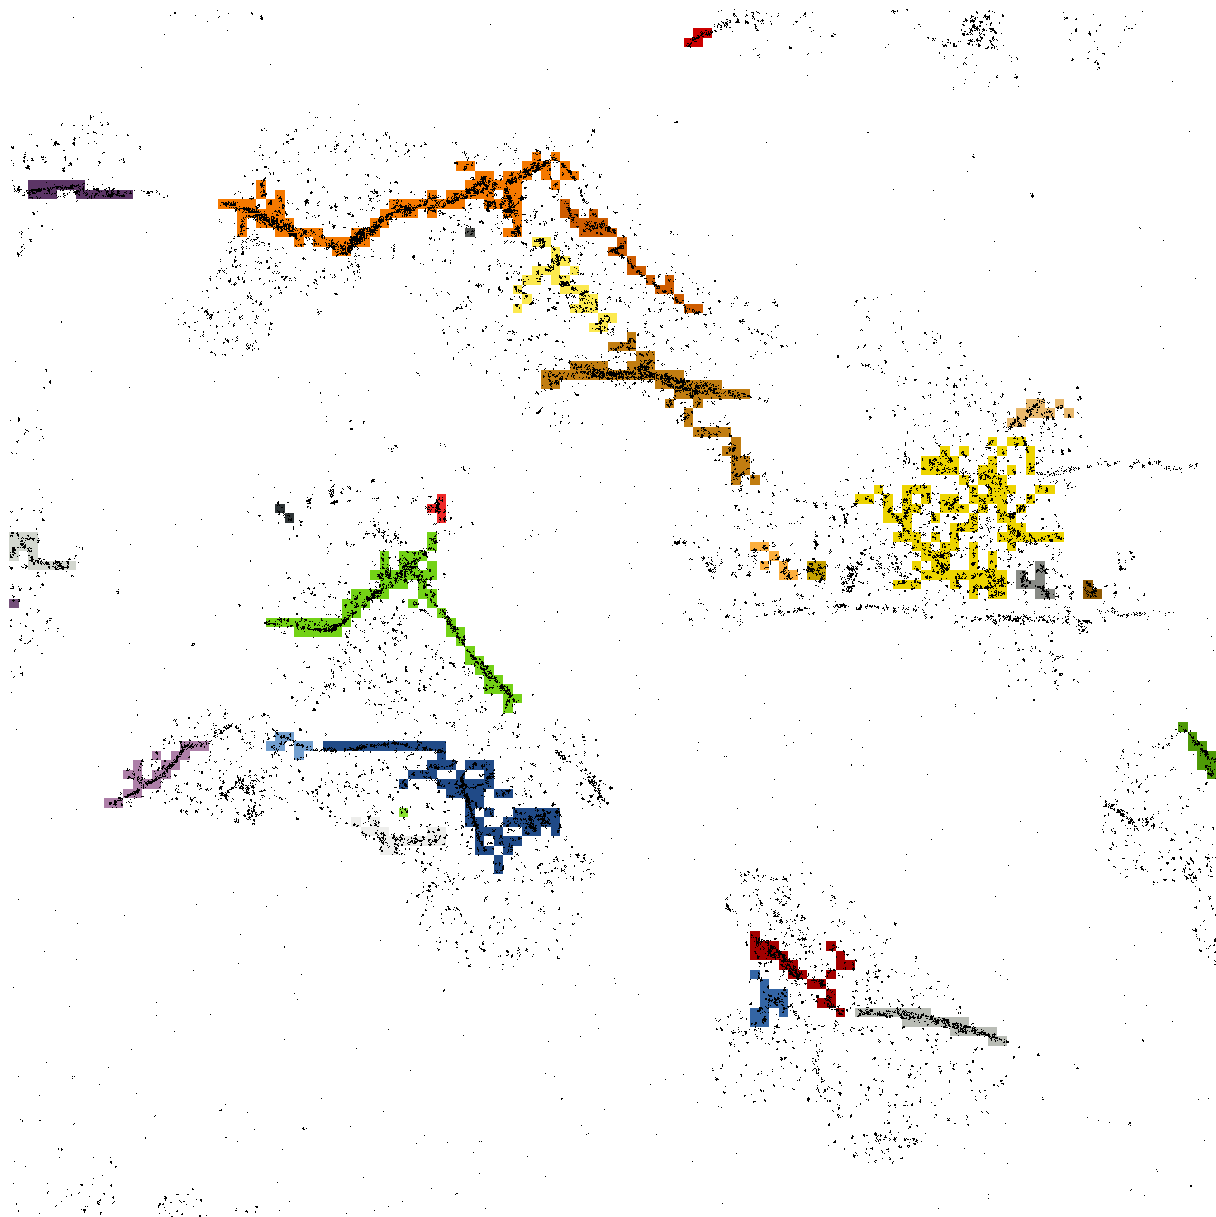
\includegraphics[width=\textwidth]{roundness-long.png}}
		\caption{}\label{fig:roundness-long.png}
	\end{subfigure}%
	\quad
	\begin{subfigure}[b]{4.2cm}
		\fbox{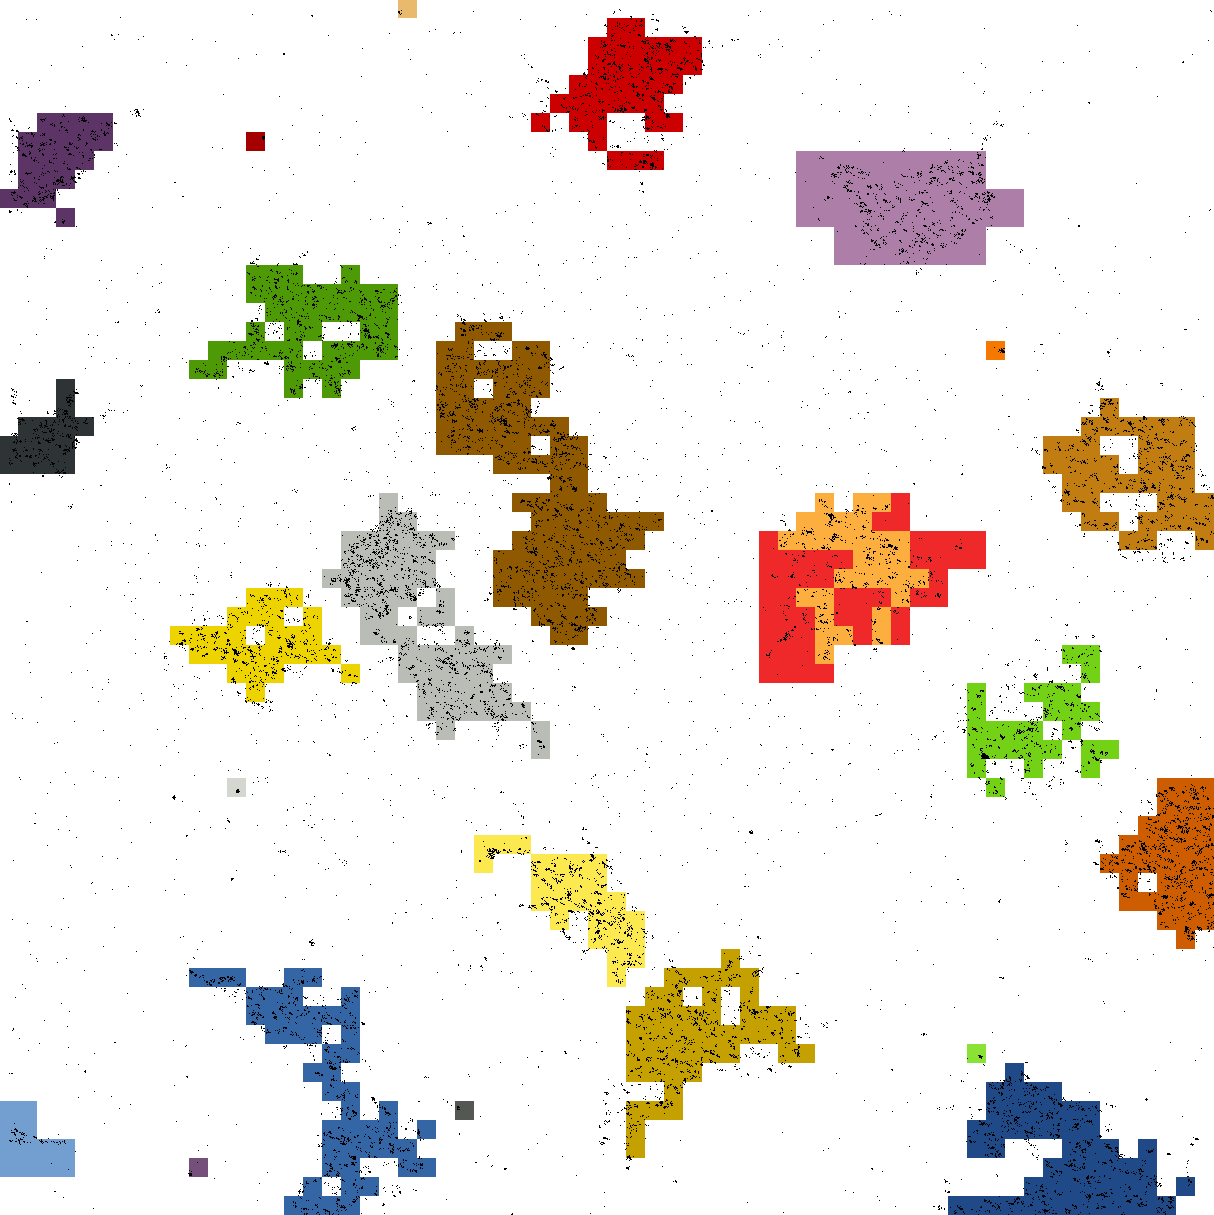
\includegraphics[width=\textwidth]{roundness-round.png}}
		\caption{}\label{fig:roundness-round.png}
	\end{subfigure}

	\caption[A comparison of roundness values.]{The general shape of the
		clusters found can be described using the roundness measure. A value
		closer to 0 means longer and thinner clusters, whereas values closer to
		1 mean clusters that are more circular.}\label{fig:roundness}
\end{figure}

\subsection{Point Analysis}
\label{sub:point_analysis}

Here, the points contained in the nodes of the quadtree that were considered
part of the cluster are considered; the nodes are only used to select the
correct points.

\subsubsection{Cluster Perimeter}
\label{ssub:cluster_perimeter_point}

\subsubsection*{Convex Hull Algorithm}
\label{ssub:Convex Hull Algorithm}

There are a number of algorithms that attempt to find the bounding polygon of a
set of points. Ignoring any holes in the cluster, the perimeter of this
bounding polygon is equivalent to the perimeter of the cluster.

The simplest method of finding this bounding polygon is using the \emph{convex
hull} method\cite{barber1996quickhull}. In principle, this involves starting
with a circle far larger than the points it encloses, which is reduced in size,
without letting any point leave the shape, until only straight lines exist
between external points. The final shape can be pictured by imagining each of
the points as a nail in a piece of wood. The convex hull algorithm then
calculates the shape that would be produced if an elastic band were stretched
around these nails.

The major disadvantage of this algorithm is that, as the name suggest, the
final shape consists only of convex angles, meaning that the actual shape of
the perimeter of the points may be lost, as shown in
Figure~\ref{fig:convex-hull}.

\begin{figure}[tbhp]
	\centering
	\includegraphics[width=5cm]{convex-hull.pdf}

	\caption[Convex versus concave hull algorithms.]{Convex versus concave hull
		algorithms. The red line shows the convex hull found for this set of
		points, which misses much of the detail and will report the area as
		being significantly above its actual value. The blue line is the
		concave hull.}\label{fig:convex-hull}
\end{figure}

\subsubsection*{Concave Hull Algorithm}
\label{ssub:Concave Hull Algorithm}

An alternative to the convex hull algorithm is the significantly more complex
\emph{concave} hull algorithm\cite{moreira2007concave}. Instead of simply
finding the outermost shape that will enclose all of the points, the concave
hull algorithm finds that shape that fits the outer boundary of the points more
closely. The steps involved are listed below.

\begin{enumerate}
	\item Find the the most southerly point to be the first point in the hull.
	\item The algorithm looks at the distance to each of the nearest $n$
		points, where $n$ is specified beforehand.
	\item From these possibilities, it chooses the closest to be added to the
		``hull''.
	\item The new line segment that would be added by joining the existing hull
		to the new point is examined to ensure that it does not cross the
		existing hull at all.
	\item If it does cross, this point is removed as a possibility of being a
		part of the hull and the next nearest point is checked.
	\item When the initial starting point is reached again, the algorithm will
		have generated a closed loop joining a number of points together.
	\item This closed loop is checked to ensure that all points lie either on
		the hull or are enclosed within it.
	\item If there are any points that fall outside the hull, the results are
		abandoned and the algorithm is re-run with the number of neighbours to
		check, $n$, incremented by one.
	\item When a hull is found that encloses all points, the algorithm
		terminates.
\end{enumerate}

Most implementations of the concave hull algorithm require an argument
specifying the number of neighbours to examine when choosing the next segment.
A higher number of neighbouring points that are checked, the less the final
hull will include small incursions into the shape and so the hull will be
smoother. The blue line in Figure~\ref{fig:convex-hull} shows the concave hull
identified for a cluster with a neighbouring number of 4.

\subsubsection*{Delaunay Triangulation}
\label{ssub:Delaunay Triangulation}

Another, more complex to implement, alternative is Delaunay
Triangulation\cite{delaunay1934sphere}. This is a method first proposed in 1934
by Boris Delaunay for use in geographical applications.

\begin{quote}
	The Delaunay triangulation is a triangulation which is equivalent to the
	nerve of the cells in a Voronoi diagram, i.e., that triangulation of the
	convex hull of the points in the diagram in which every circumcircle of a
	triangle is an empty circle.\\
	\hspace*{\fill}\cite{okabe2009spatial}
\end{quote}

This means that the result is a densely connected graph where every point is
joined to exactly two other points such that there are no points within the
circle joining any three connected points. This has the side effect of
calculating the convex hull and makes calculating the area of the cluster
simple---the areas of the triangles are summed.

This method is not used to calculate the perimeter or the area since the
implementation is generally more complex than other methods and provides more
information than is useful, and hence takes longer to calculate. Finally the
area of the cluster that is identified is convex and so shows the same issues
as the convex hull algorithm above.

\subsubsection{Cluster Area}
\label{ssub:cluster_area_point}

If using a hull-based algorithm to find the perimeter of the cluster, once the
perimeter hull has been identified, it is simple to calculate the area enclosed
by that cluster. Since the hull consists only of straight lines
connecting single points, the area can be calculated by splitting the polygon
into regular triangles, and finding each of their areas individually. The area
of the whole cluster is then given by the sum of these areas. An algorithm for
calculating the area of the irregular polygon produced with this method is
shown in Listing~\ref{lst:polygon-area}.

\begin{center}
\begin{minipage}{\textwidth}
	\begin{lstlisting}[caption={[Code to find the area of an irregular
	polygon.]Code to find the area of an irregular polygon.  Adapted
	from~\cite{finley2006poly}}, label=lst:polygon-area] public
	|polygonArea(points, numPoints)| {

		area = 0;
		j = numPoints - 1;

		/* Sum the area contained between each pair of points
		 * and the y-axis on the right hand side of the shape
		 * and subtract the area between pairs of points and
		 * the y-axis on the left hand side.
		 */
		for (i=0; i < numpoints; i++) {
			area += (points[j].getX() + points.[i].getX()) *
		        	(points[j].getY() - points.[i].getY());
			j = i;
		}
		return area/2;
	}
\end{lstlisting}
\end{minipage}
\end{center}

\subsection{Dilate/Erode Alternative}
\label{ssub:Dilate/Erode Alternative}

As an alternative to the other methods described above, a fast technique for
finding the perimeter and area of the points that takes advantage of the fact
that the points are represented in an image in ImageJ was developed. With the
points that represent the cluster to find the details for, and using the
built-in commands in ImageJ, several successive dilate filters are applied to
the points followed by the same number of erode filters.

\paragraph{Dilate Filter}
\label{par:dilate_filter}

A dilate filter, also known as a grow or expand filter, is a technique in
mathematical morphology to extend the boundaries of a shape by adding pixels to
the outer edge. It can be performed only on a binary image since the pixels
that are added must all have the same value. The filter adds new white
foreground pixels to the boundary of existing foreground regions with the
effect that shapes get larger and holes in those shapes are reduced.

\paragraph{Erode Filter}
\label{par:erode_filter}

An erode filter, also called a shrink or reduce filter, is a very similar
process to dilation above, but in reverse. Instead of adding to foreground
regions, pixels are removed. Another way to consider the erode filter is as an
identical filter to dilating but performed on the black background pixels.

In order to get the usful information using this method, the dilate filter is
applied $N$ times. This has the effect of filling in holes that exist
between points and combining the cluster into a single conglomerate that can be
manipulated as a one object, rather than a number of distinct points. Next an
erode filter is applied to the shape $N+1$ times. This reduces the shape back
to the original size of the points. The reason for the extra erode is to remove
outlying points that were not joined in to the main shape and so would skew the
results. Finally, an additional dilation is performed to reverse the effect of
the extra erode.

Figure~\ref{fig:dilate-erode} shows these steps on a number of points that have
been identified, \subref{fig:de0}, which is dilated twice, \subref{fig:de1} and
\subref{fig:de2}, before being eroded again, \subref{fig:de3} to
\subref{fig:de5} and then dilated again, \subref{fig:de6}. It can be seen from
the image that the shape in \subref{fig:de6} is a good approximation of the
outline of the points in \subref{fig:de0} with the single outlying point
removed.

\begin{figure}[tbhp]
	\centering
	\begin{subfigure}[b]{2cm}
		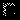
\includegraphics[width=\textwidth]{dilate-erode-0.png}
		\caption{}\label{fig:de0}
	\end{subfigure}%
	\quad
	\begin{subfigure}[b]{2cm}
		
\includegraphics[width=\textwidth]{dilate-erode-1.png}
		\caption{}\label{fig:de1}
	\end{subfigure}%
	\quad
	\begin{subfigure}[b]{2cm}
		
\includegraphics[width=\textwidth]{dilate-erode-2.png}
		\caption{}\label{fig:de2}
	\end{subfigure}
	\quad
	\begin{subfigure}[b]{2cm}
		
\includegraphics[width=\textwidth]{dilate-erode-3.png}
		\caption{}\label{fig:de3}
	\end{subfigure}
	\quad \\[1em]
	\begin{subfigure}[b]{2cm}
		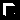
\includegraphics[width=\textwidth]{dilate-erode-4.png}
		\caption{}\label{fig:de4}
	\end{subfigure}
	\quad
	\begin{subfigure}[b]{2cm}
		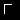
\includegraphics[width=\textwidth]{dilate-erode-5.png}
		\caption{}\label{fig:de5}
	\end{subfigure}
	\quad
	\begin{subfigure}[b]{2cm}
		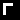
\includegraphics[width=\textwidth]{dilate-erode-6.png}
		\caption{}\label{fig:de6}
	\end{subfigure}
	\quad
	\begin{subfigure}[b]{2cm}
		
\includegraphics[width=\textwidth]{dilate-erode-7.png}
		\caption{}\label{fig:de7}
	\end{subfigure}
	\caption{}\label{fig:dilate-erode}
\end{figure}

To find the area now becomes a simple case of counting the number of white
pixels that are left in the image and then scaling this according to the scale
factor used to draw the image (page~\pageref{it:scale}). A final step is
performed to get the perimeter of the shape. This time an outline filter is
applied. This has the effect of creating a one pixel wide outline of the shape.
The perimeter is then the length of this outline which, again, can be found by
counting the pixels it consists of and scaling for the size of the pixels.

% TODO sentence to say the image is complete tada etc.
